% 2001 年全国旧课程卷文科第 18 题：直角梯形底面的四棱锥
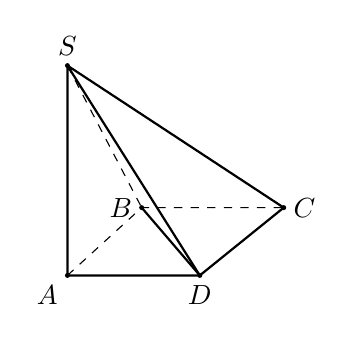
\begin{tikzpicture}[>=stealth, scale=0.82]
  \coordinate (A) at (0,0);
  \coordinate (B) at (1.15,1.05);
  \coordinate (C) at (3.35,1.05);
  \coordinate (D) at (2.05,0);
  \coordinate (S) at (0,3.25);

  \draw[thick] (S)--(A) (S)--(C) (S)--(D);
  \draw[dashed] (S)--(B);
  \draw[thick] (A)--(D)--(C);
  \draw[dashed] (A)--(B)--(C);
  \draw[thick] (B)--(D);

  \fill (S) circle (1.1pt) node[above] {$S$};
  \fill (A) circle (1.1pt) node[below left] {$A$};
  \fill (B) circle (1.1pt) node[left] {$B$};
  \fill (C) circle (1.1pt) node[right] {$C$};
  \fill (D) circle (1.1pt) node[below] {$D$};
\end{tikzpicture}
